
        \section{Demonstration project}
        The aim of the demonstration project is to provide an easy way to explore
        the IDE without reading long documents. The
        demonstration project can be opened from the welcome dialog ( Main Menu
        Help Welcome dialog Open demonstration project. )
        Demonstration project should introduce new user into usage of the most
        common functions of the IDE like assembling the code, running simulator
        and so on. Demonstration project cannot be modified by the user in order
        to make it less volatile.
                \begin{figure}
                    \centering{}
                    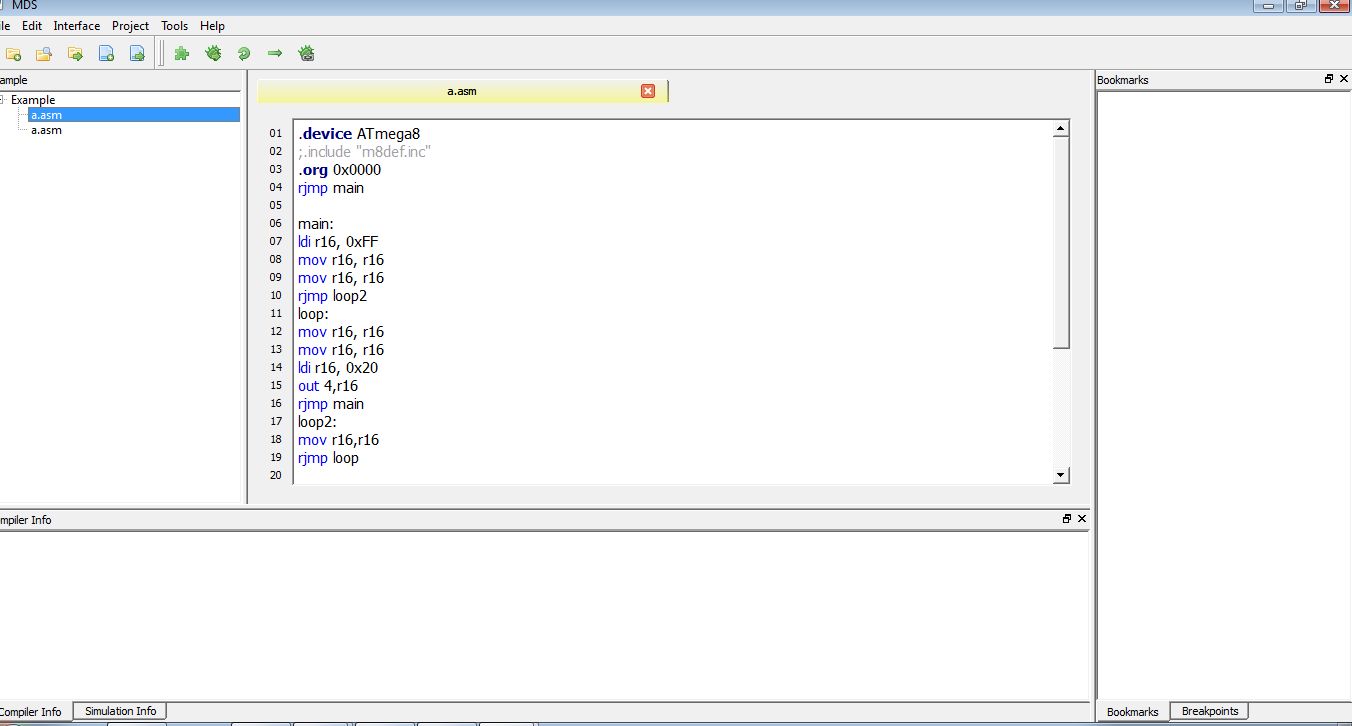
\includegraphics [scale=0.4]{img/Demonstration_project.png}
                    \caption{Demonstration project}
                \end{figure}
        \section{Your first project}

        \section{What is PicoBlaze?}
        PicoBlaze is the designation of a series of three free soft processor cores
        from Xilinx for use in their FPGA and CPLD products. They are based on a RISC
        architecture of 8 bits and can reach speeds up to 100 MIPS on the Virtex 4
        FPGA"s family. The processors have an 8-bit address and data port for access
        to a wide range of peripherals. The license of the cores allows their free
        use, albeit only on Xilinx devices, and they come with development tools.
        All instructions execute in two clock cycles, making performance of the core instruction
        set deterministic. Interrupt response is not more than five clock cycles. As a resource
        optimization, it is possible for two PicoBlaze cores to share the same 1k x 18 instruction
        PROM, taking advantage of the dual-ported implementation of this block on Xilinx FPGAs.

                \subsection{PicoBlaze features:}
                        \begin{itemize}
                                \item 16 byte-wide general-purpose data registers
                                \item 1K instructions of programmable on-chip pr
                                        ogram store, automatically loaded during
                                        FPGA configuration
                                \item Byte-wide Arithmetic Logic Unit (ALU) with CARRY and ZERO indicator flags
                                \item 64-byte internal scratchpad RAM
                                \item 256 input and 256 output ports for easy expansion and enhancement
                                \item Automatic 31-location CALL/RETURN stack
                                \item Predictable performance, always two clock cy
                                        cles per instruction, up to 200 MHz or
                                        100 MIPS in a Virtex-II Pro FPGA
                                \item Fast interrupt response; worst-case 5 clock cycles
                                \item Optimized for Xilinx Spartan-3, Virtex-II, and Virtex-II Pro FPGA architectures just
                                        96 slices and 0.5 to 1 block RAM
                                \item Assembler, instruction-set simulator support
                        \end{itemize}
